
\section{Obstacle Avoidance}


Obstacle avoidance is a crucial component of coverage path planning (CPP), applicable in various contexts such as agricultural fields, warehouses, and more. In agricultural fields, static obstacles include trees, rocks, houses, and other structures, collectively referred to as keep-out zones. Obstacles are represented as polygons of various shapes and sizes, which the robot must avoid and all the obstacle information is available beforehand. 

\vspace{3mm}  

One of the critical aspects of the CPP algorithm is its efficiency in obstacle avoidance. Given that the robot will encounter obstacles multiple times during its operation, it is essential that the algorithm minimizes the computation time required for each avoidance maneuver. The algorithm should be optimized to quickly navigate around obstacles. Path adjustments must be computed swiftly to ensure minimal disruption to the overall coverage path. 


\vspace{3mm}  


The obstacle avoidance algorithm in coverage path planning (CPP) consists of two main components:

\begin{enumerate}
    \setlength\itemsep{0em}
    \item Setup and dynamic grid generation.
    \item Path validity checking and obstacle free path generation.
\end{enumerate}

\subsection{Setup and Dynamic Grid Generation}

The initial setup begins once the algorithm receives all the data. The first crucial step is to account for the robot's physical dimensions by creating a configuration space. This ensures that the algorithm considers the robot's actual operating space, not just a point in the field.

\vspace{3mm}  

CPP operates in continuous space for path planning, but representing obstacles solely in continuous space is computationally prohibitive, especially in obstacle-rich environments. On the other hand, completely using discrete space is impractical for large fields, such as agricultural areas, because methods like occupancy grids would be too expensive to generate and manage over extensive areas.

\vspace{3mm}  

To address this, a hybrid approach is adopted. Continuous space is used for general path planning, while obstacles are represented in both continuous and discrete spaces. Discrete space involves creating separate occupancy grids for each obstacle. A critical challenge here is determining the size of the grid cells: they must be small enough to accurately represent the obstacle yet large enough to avoid excessive computational load. The algorithm addresses this by generating dynamic grids based on the size of the obstacle and the robot's non-holonomic constraints.

\vspace{3mm}  

\textbf{Dynamic Grid Generation:}
The initial objective is to dynamically generate an occupancy grid for each obstacle. The algorithm begins by extending the vertices of each polygonal obstacle to create a safe zone around it. This extended obstacle is then approximated as a rectangle using the minimum and maximum coordinates of the extended polygon.

\vspace{3mm}  

To generate the grid for this approximated obstacle, the algorithm considers the robot's non-holonomic constraints. It calculates a curve using the two extreme angles of the vision cone and a step length, ensuring the robot can navigate this curve with the minimum turning radius until a 90-degree turn is achieved. At this point, the changes in the x and y coordinates (dx and dy) are recorded. These values are used to determine the grid's dimensions, with an allowance of 1.5 times the curve distance along the robot's heading and half the obstacle's width. This setup ensures that the robot can navigate around the obstacle even with its non-holonomic constraints. 

\vspace{3mm}  

The non-holonomic constraints used for grid generation and generated grids based on obstacle dimensions are illustrated in \autoref{fig:Dynamic_Grid_Generation}. The pseudocode for the dynamic grid generation for each obstacle is provided in (Algorithm \autoref{alg:setup_obstacle_algorithm})


% selected field region.
\begin{figure}[H]
    \centering
    \begin{tabular}{cc} 
        \begin{subfigure}{0.5\textwidth}
            \centering
            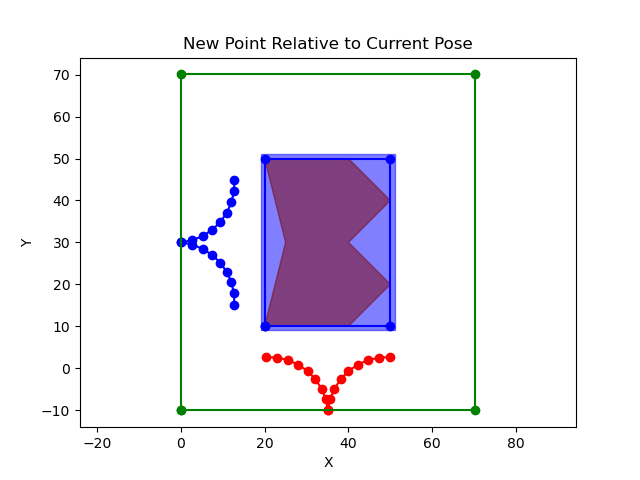
\includegraphics[width=\textwidth]{Images/Algorithm_obs/Grid/new_ob1.png}
            % \caption{Selected Field Region}
        \end{subfigure} 
        &
        \begin{subfigure}{0.5\textwidth}
            \centering
            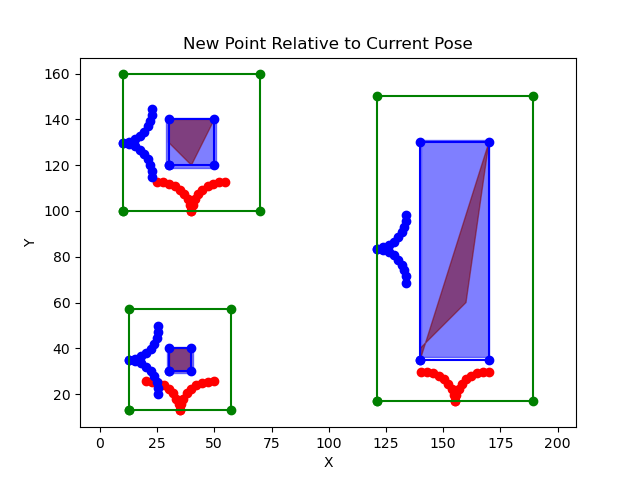
\includegraphics[width=\textwidth]{Images/Algorithm_obs/Grid/multi_obs.png}
            % \caption{Points in the Region (Green)}
        \end{subfigure}
    \end{tabular}
    \caption{Dynamic Grid Generation.\label{fig:Dynamic_Grid_Generation}} 
\end{figure}

In the figure, the filled shape represents an obstacle. The red and blue curves depict the robot's minimum turning radius. The blue rectangular region indicates the extended and approximated obstacle area, while the green rectangle represents the generated grid for the obstacle.

\vspace{3mm}  

Convention to be followed for the Obstacle Avoidance Algorithm:
\begin{multicols}{2}
\begin{itemize}[noitemsep,topsep=0pt]
    \item $OB$: Obstacle.
    \item $OB_p$: Polygonal obstacles.
    \item $OB_e$: Extended obstacles.
    \item $g$: grid.
    \item $g_s$: grids.
    \item $p_{bu}$: Buffer points.
    \item $SP$: Salient Point.
    \item $P_{re}$: Remaining path.
\end{itemize}
\end{multicols}
    
\vspace{3mm}  

Notations for the Dynamic Grid Generation Algorithm:
\begin{itemize}[noitemsep,topsep=0pt]
    \item $dx$: Distance in the x direction at 90degree turn.
    \item $dy$: Distance in the y direction at 90degree turn.
    \item $fd$: Free grid space from the obstacle edge.  
\end{itemize}

\begin{algorithm}[H]
    \caption{DynamicGridAlgorithm}
    \label{alg:setup_obstacle_algorithm}
    \begin{algorithmic}[1]
    \Statex \textbf{Input:} polygonal obstacles ($OB_p$), grid diameter ($g_d$), vision cone ($VC$), safe margin ($sm$)
    \Statex \textbf{Output:} Extended polygonal obstacles ($OB_e$), grids ($g_s$), buffer points ($p_{bu}$)
    \newline
    \State $dx, dy \leftarrow$ ComputeDistancesFor90DegreeTurn($VC$)
    \State $fd \leftarrow 1.5 \times dy$
    \State $OB_e \leftarrow$ ExtendPolygonForSafeMargin($OB_p$, $sm$)
    \State $g_s \leftarrow$ ComputeGrid($OB_e$, $g_d$, $fd$)
    \State $p_{bu} \leftarrow$ PointsSurroundingObstacles($OB_e$)
    \State \Return $OB_e$, $g_s$, $p_{bu}$
    \end{algorithmic}
    \end{algorithm}

\vspace{3mm}  


Once the grid size is determined, the grid cells are generated. The cell size is chosen based on the robot's dimensions: larger robots do not require fine grids as they cannot move cell by cell. Therefore, an appropriate grid cell size is selected to suit the robot's size. For each obstacle, point data (centers of the complete grid) is generated over the occupancy grid. The algorithm extracts points around the obstacle's boundary, known as buffer points. These buffer points help in navigating around the obstacles efficiently.



\subsubsection{Path validity checking and obstacle free path generation}

This section outlines the second phase of the obstacle avoidance algorithm, focusing on the real-time aspects of navigation once the initial setup is complete. After setting up the obstacles and generating the dynamic grids, the algorithm proceeds with the regular behavioral approach for path planning. The pseudocode for the complete algorithm with obstacles is shown in (Algorithm \autoref{alg:complete_behavioral_obstacle_avoidance})





\begin{algorithm}[H]
    \caption{CompleteBehavioralObstacles}
    \label{alg:complete_behavioral_obstacle_avoidance}
    \begin{algorithmic}[1]
    \Statex \textbf{Input:} 2D points ($p_{2d}$), initial robot pose ($r_{\text{pos}}$), turning radius ($R_{\text{tu}}$), polygonal obstacles ($OB_p$), grid diameter ($g_d$), vision cone ($VC$) 
    \Statex \textbf{Output:} Dubins path $P_{cd}$
    \newline
    \State $OB_e, g_s, p_{bu} \leftarrow$ SetupObstacles($OB_p$, $g_d$, $VC$, $sm$)
    \State $p_{cl}, \delta_{\text{bc}} \leftarrow$ CentroidsAndAutoBehaviorShift($P_{2d}$, $R_{\text{min}}$, $R_{\text{max}}$, $N$ )
    \State $p_r \leftarrow p_{cl}$
    \State $\delta_c \leftarrow 0$
    \State $P_c \leftarrow []$
    
    \While{True}
        \If{$\delta_c <  \delta_{\text{bc}}$}
            \State $P_s, p_r \leftarrow$ Behavior\_1($OB_e$, $g_s$, $p_{bu}$, $p_r$, $P_{cl}$, $N_s$, $r_{\text{pos}}$, $VC$, $C$, $R_{\text{conc}}$, $step$)
        \Else
            \State $P_s, p_r \leftarrow$ Behavior\_2($OB_e$, $g_s$, $p_{bu}$, $p_r$, $P_{cl}$, $N_s$, $r_{\text{pos}}$, $VC$, $C$, $R_{\text{conc}}$, $step$)
        \EndIf
        
        \State $P_c \mathrel{+}= P_s$
        \State $r_{\text{pos}} \leftarrow P_c[-1]$
        \State $\delta_c \leftarrow$ UpdateCoveragePerc($P_c$, $p_r$)
        
        \If{$\text{len}(P_s) == 0$}
            \State \textbf{break}
        \EndIf
    \EndWhile
    
    \State $P_d \leftarrow$ DubinsPath($P_c$, $R_{\text{tu}}$)
    \State $P_{re} \leftarrow$ PathAroundObstaclesAlgorithm($OB_e$,$P_r$, $r_{pos}$, $R_{tu}$)
    \State $P_{cd} \leftarrow P_d + P_{re}$

    \State \Return $P_{cd}$
    \end{algorithmic}
\end{algorithm}


The path generation process begins as described previously. However, this time, the algorithm includes a mechanism to detect path collisions with obstacles. If no obstacles are detected along the planned path, the behavioral algorithm operates normally. When an obstacle is detected, the algorithm initiates a sequence of steps to navigate around it. The pseudocode for the behavior 1 and behavior 2 with the inclusion of path validity check is shown in (Algorithm \autoref{alg:behavioral1_obs}) and (Algorithm \autoref{alg:behavioral_algorithm_2_obs}) respectively.

\vspace{3mm}  



Description of the notations:
\begin{itemize}[noitemsep,topsep=0pt]
    \item $P_{cu}$: Current path
    \item $P_{OB free}$: Obstacle free path
\end{itemize}

\begin{algorithm}[H]
    \caption{Behavior\_1\_with\_Obstacles}
    \label{alg:behavioral1_obs}
    \begin{algorithmic}[1]

    \Statex \textbf{Input:} Extended polygonal obstacles ($OB_e$), grids ($g_s$), buffer points ($p_{bu}$), 2D points ($P_{2d}$), clustered points ($p_{cl}$), number of sample orientations ($N_s$), robot pose ($r_{pos}$), vision cone ($VC$), centroid ($C$), concurrent region radii ($R_{\text{conc}}$), step size ($S$)

    \Statex \textbf{Output:} Complete straight path $P_{cs}$, remaining points $p_r$
    \newline
    \State $P_{cs} \leftarrow []$
    \State $P_t \leftarrow [[] \text{ for } \_ \text{ in range}(N_s)]$
    \State $p_{co} \leftarrow [[] \text{ for } \_ \text{ in range}(N_s)]$
    \State $O_{sa} \leftarrow$ SampleTheOrientations($R_{pos}[2]$, $N_s$, $S$)
    
    \For{$i, O$ \textbf{in} $O_{sa}$}
        \State $R_{pos}[2] \leftarrow O$
        \While{no point is visible}
            \State $p_v \leftarrow$ ComputeVisionConePoints($r_{pos}$, $VC$)
            \State $p_{po} \leftarrow$ FindPotentialPoint($r_{pos}$, $p_v$)
            \If{$p_{po}$ is None}
                \State \textbf{break}
            \EndIf
            \State $O_n \leftarrow$ FromCurrentPoseToPotentialPoint($r_{pos}$, $p_{po}$)
            \State $P_{cu} \leftarrow$ [[$r_{pos}$, $p_{po}$]]
            \State $P_{OB free} \leftarrow$ ComputeObstacleFreePath($P_{cu}$, $O_n$)


            \State $P_t[i] \mathrel{+}= P_{OB free}$
            
            \State $p_{int} \leftarrow$ CheckIntermediatePoints($p_r$)
            \State $P_t[i].\text{append}(p_{int})$
            \State $p_c[i].\text{append}(\text{len}(P_t))$
            \State $p_r \leftarrow p_{cl} - P_t$
            \State $r_{pos} \leftarrow P_{OB free}[-1]$
        \EndWhile
    \EndFor
    
    \State $O_{bi} \leftarrow \text{argmax}(p_c[:])$
    \State $P_{cs} \leftarrow P_t[O_{bi}]$
    
    \State $r_{pos} \leftarrow P_{cs}[-1]$
    \State $p_{tu} \leftarrow$ PotentialPointToTurn($p_r$, $R_{\text{conc}}$, $r_{pos}$)
    \State $O_b \leftarrow$ TowardsCentroid($p_{tu}$, $C$)

    \State $P_{cu} \leftarrow$ [[$r_{pos}$, $p_{tu}$]]
    \State $P_{OB free} \leftarrow$ ComputeObstacleFreePath($OB_e$, $g_s$, $p_{bu}$, $P_{cs}$, $P_{cu}$, $O_b$)

    \State $P_{cs} \mathrel{+}= P_{OB free}$
    \State $p_r.\text{remove}([P_{OB free}])$ 
    
    \State \Return $P_{cs}$, $p_r$
    \end{algorithmic}
    \end{algorithm}




    









\begin{algorithm}[H]
    \caption{Behavioral\_2\_with\_Obstacles}
    \label{alg:behavioral_algorithm_2_obs}
    \begin{algorithmic}[1]

    \Statex \textbf{Input:} Extended polygonal obstacles ($OB_e$), grids ($g_s$), buffer points ($p_{bu}$), 2D points ($P_{2d}$), clustered points ($p_{cl}$), number of sample orientations ($N_s$), robot pose ($r_{pos}$), vision cone ($VC$), centroid ($C$), concurrent region radii ($R_{\text{conc}}$), step size ($S$)

    \Statex \textbf{Output:} Complete straight path $P_{cs}$, remaining points $p_r$
    \newline
    \State $P_{cs} \leftarrow []$
    \State $P_t \leftarrow [[] \text{ for } \_ \text{ in range}(N_s)]$
    \State $p_{co} \leftarrow [[] \text{ for } \_ \text{ in range}(N_s)]$
    \State $O_{sa} \leftarrow$ SampleTheOrientations($R_{pos}[2]$, $N_s$, $S$)
    
    \For{$i, O$ \textbf{in} $O_{sa}$}
        \State $R_{pos}[2] \leftarrow O$
        \While{no point is visible}
            \State $p_v \leftarrow$ ComputeVisionConePoints($r_{pos}$, $VC$)
            \State $p_{po} \leftarrow$ FindPotentialPoint($r_{pos}$, $p_v$)
            \If{$p_{po}$ is None}
                \State \textbf{break}
            \EndIf
            \State $O_n \leftarrow$ FromCurrentPoseToPotentialPoint($r_{pos}$, $p_{po}$)
            \State $P_{cu} \leftarrow$ [[$r_{pos}$, $p_{po}$]]
            \State $P_{OB free} \leftarrow$ ComputeObstacleFreePath($P_{cu}$, $O_n$)


            \State $P_t[i] \mathrel{+}= P_{OB free}$
            
            \State $p_{int} \leftarrow$ CheckIntermediatePoints($p_r$)
            \State $P_t[i].\text{append}(p_{int})$
            \State $p_c[i].\text{append}(\text{len}(P_t))$
            \State $p_r \leftarrow p_{cl} - P_t$
            \State $r_{pos} \leftarrow P_{OB free}[-1]$
        \EndWhile
    \EndFor
    
    \State $O_{bi} \leftarrow \text{argmax}(p_c[:])$
    \State $P_{cs} \leftarrow P_t[O_{bi}]$
    
    \State $r_{pos} \leftarrow P_{cs}[-1]$

    \State $p_{tu} \leftarrow$ PotentialPointToTurnCCW($p_r$, $R_{\text{conc}}$, $r_{pos}$)
    \State $O_b \leftarrow$ VectorsTowardsNextCCWPoint($p_{tu}$, $p_r$)


    \State $P_{cu} \leftarrow$ [[$r_{pos}$, $p_{tu}$]]
    \State $P_{OB free} \leftarrow$ ComputeObstacleFreePath($OB_e$, $g_s$, $p_{bu}$, $P_{cs}$, $P_{cu}$, $O_b$)

    \State $P_{cs} \mathrel{+}= P_{OB free}$
    \State $p_r.\text{remove}([P_{OB free}])$ 
    
    \State \Return $P_{cs}$, $p_r$
    \end{algorithmic}
    \end{algorithm}

\subsection{Collision Detection and Salient Point Identification}


Upon detecting an obstacle in the path, the algorithm first identifies a line along the robot’s heading and checks for intersection points with the obstacle. At this stage, buffer points previously defined around the obstacle become critical. The algorithm identifies the furthest buffer point along the robot's heading, which marks the end of the line. It then calculates the perpendicular distances from this line to all buffer points, selecting two points on either side of the line at the maximum distance. These points are designated as salient points, serving as key navigational targets to avoid the obstacle.

\vspace{3mm}  

Once the salient points are determined, they become the goal points for the robot to bypass the obstacle. The robot's current position is the starting point for this avoidance maneuver. The algorithm then checks whether the robot is inside the grid. If the robot is outside the grid, the salient points are directly used as goal points, and the robot navigates towards them following its non-holonomic constraints. The grid is designed such that if the robot is at the edge, it can avoid the obstacle by reaching these extreme points directly.

\vspace{3mm}  

The \autoref{fig:salient_points_obs} illustrates the selection of salient points based on the robot's orientation when the path intersects with an obstacle. In the figure, dark blue points denote grid centers, red and black points mark grid centers within the obstacle, and green points indicate buffer points. The yellow point signifies the extreme end of the robot's orientation, while the purple direction represents the robot's orientation. Light blue points indicate the region of interest, and the two dark purple points at the extreme corners of the obstacle represent the salient points.

% Include an image
\begin{figure}[H]
    \centering
    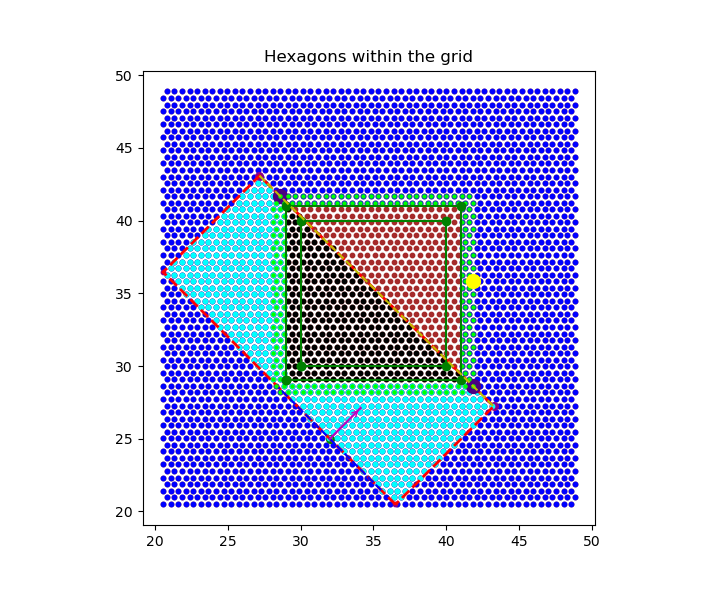
\includegraphics[width=0.5\textwidth]{Images/Algorithm_obs/Grid/salinet_point3.png}
    \caption{Selection of Salient Points.}
    \label{fig:salient_points_obs} 
\end{figure} 

\subsection{Graph-Based Path Finding}

If the robot is inside the grid, a more complex process ensures that the robot can reach the salient points while adhering to its motion constraints. A graph-based approach is utilized to find the shortest and feasible path from the robot's current position to the salient points using the grid cells.

\vspace{3mm}  

Efficient and rapid graph generation is crucial, as this process must occur each time an obstacle is encountered. The algorithm employs two extreme angles of the vision cone and a step length to create the graph. Each iteration produces a new generation of grid cells. For instance, if the robot occupies one cell, the next generation, based on the two extreme angles and step length, will occupy two cells. Subsequent generations expand similarly, covering more cells until the goal point is included in the graph.

\vspace{3mm}  

One challenge in this graph-based approach is balancing the step length. If the step length is too short, the graph requires many generations to reach the goal point, increasing computational time. Conversely, if the step length is too long, the graph may become sparse, risking the possibility of not adequately covering the goal point and potentially passing through it.


\vspace{3mm}  





To ensure an efficient and adaptive approach to obstacle avoidance, the algorithm dynamically determines the step length for graph generation. By allowing the algorithm to decide the step length, it can find a near-optimal length that generates a sparse graph initially, gradually becoming denser as it approaches the goal point. This adaptive strategy optimizes computational efficiency while ensuring thorough coverage.

\vspace{3mm}  

Automating the selection of step length involved an experimental analysis to understand its dependence on various parameters. Notably, the distance to the salient point emerged as a significant factor. By conducting experiments with different salient point positions and step lengths, a linear relationship between the distance and step length was identified. Consequently, the algorithm fits a line to this data at the outset, enabling it to automatically determine the dynamic step length based on the distance to the salient point. This near-optimal step length encourages the algorithm to generate a sparse graph initially, gradually densifying it as it approaches the goal point. This approach significantly enhances computational efficiency. The effect of step length on graph generation is illustrated in \autoref{fig:step_length}.

% selected field region.
\begin{figure}[H]
    \centering
    \begin{subfigure}{0.3\textwidth}
        \centering
        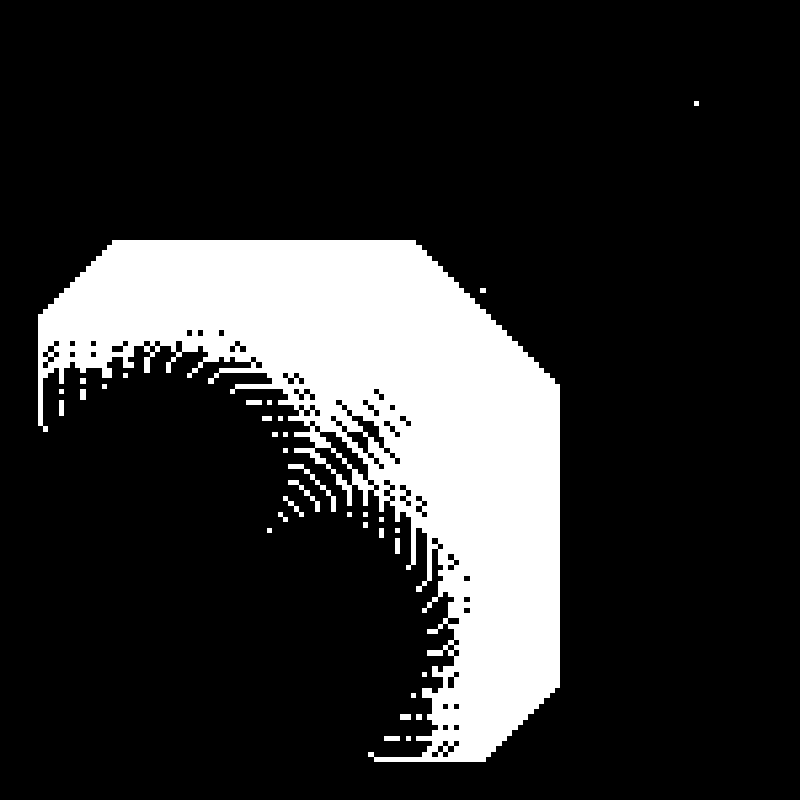
\includegraphics[width=\textwidth]{Images/Algorithm_obs/graph/Setting_step_length_for_graph_generation/60_dist_4_step_len_time_5.54_under.png}
        \caption{Step length 4.0 cm at Generation 20.}
    \end{subfigure} 
    \hfill
    \begin{subfigure}{0.3\textwidth}
        \centering
        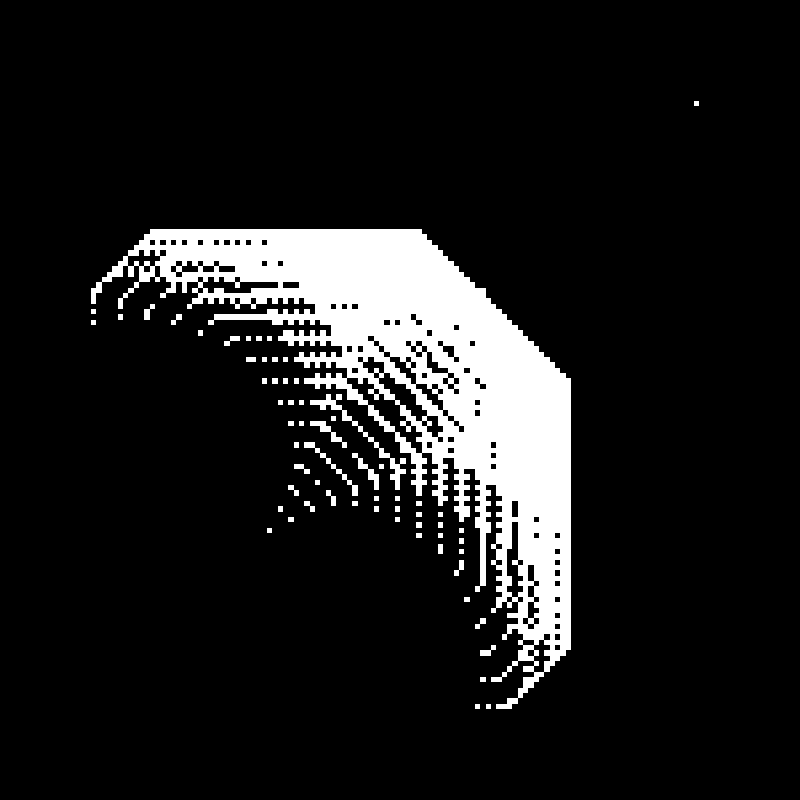
\includegraphics[width=\textwidth]{Images/Algorithm_obs/graph/Setting_step_length_for_graph_generation/60_dist_4.96_step_len_time_0.47_perfect.png}
        \caption{Step length 4.96 cm at Generation 10.}
    \end{subfigure}
    \hfill
    \begin{subfigure}{0.3\textwidth}
        \centering
        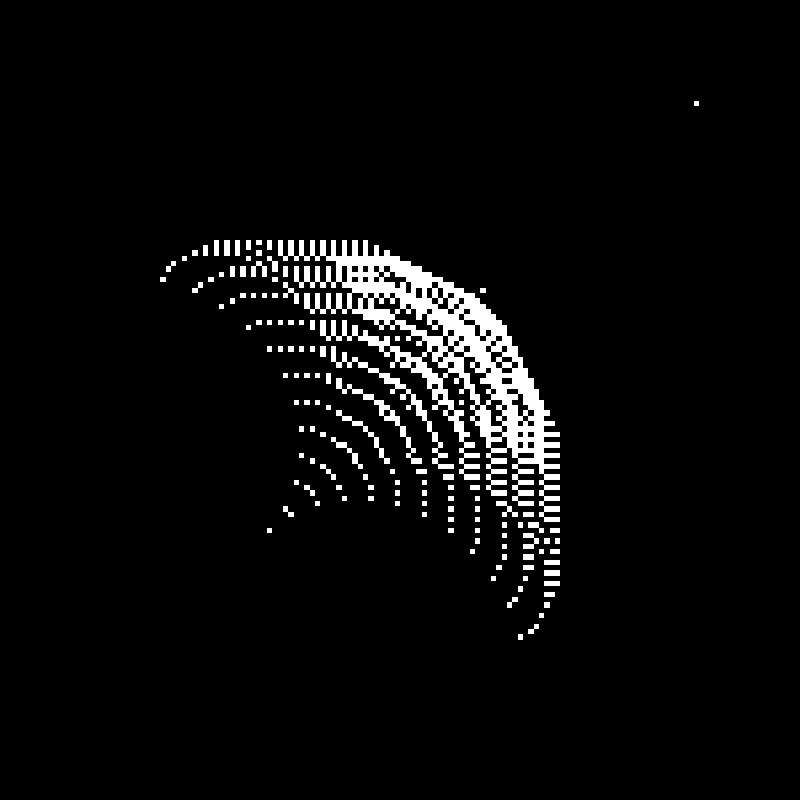
\includegraphics[width=\textwidth]{Images/Algorithm_obs/graph/Setting_step_length_for_graph_generation/60_dist_6.0_step_len_0.11_over.png}
        \caption{Step length 6.0 cm at Generation 8.}
    \end{subfigure}
    \caption{The Effect of Step Length on Graph Generation.\label{fig:step_length}} 
\end{figure}


Once the graph is generated, multiple paths from the robot's position to the salient point are available. The algorithm employs an A* search over the graph to find the shortest path. The intermediate points along this path serve as the route to avoid the obstacle and reach the goal point efficiently and swiftly. Subsequently, the regular behavior resumes for further coverage of the designated points.

\vspace{3mm}  

An example of graph generation and pathfinding is illustrated in \autoref{fig:graph_generation}. In \autoref{fig:graph_generation}a, the scenario with salient points is depicted. The while square represents the obstacle, two corner white points represent the salient points and the lower left white point denotes the robot oriented at a 45-degree angle. In \autoref{fig:graph_generation}b, the graph generation is shown. Initially, the graph is sparse and as it approaches the goal point, it becomes denser due to automatic step length selection. In \autoref{fig:graph_generation}c, the shortest path from the robot to the goal point is found using A* search over the generated graph.


% selected field region.
\begin{figure}[H]
    \centering
    \begin{subfigure}{0.3\textwidth}
        \centering
        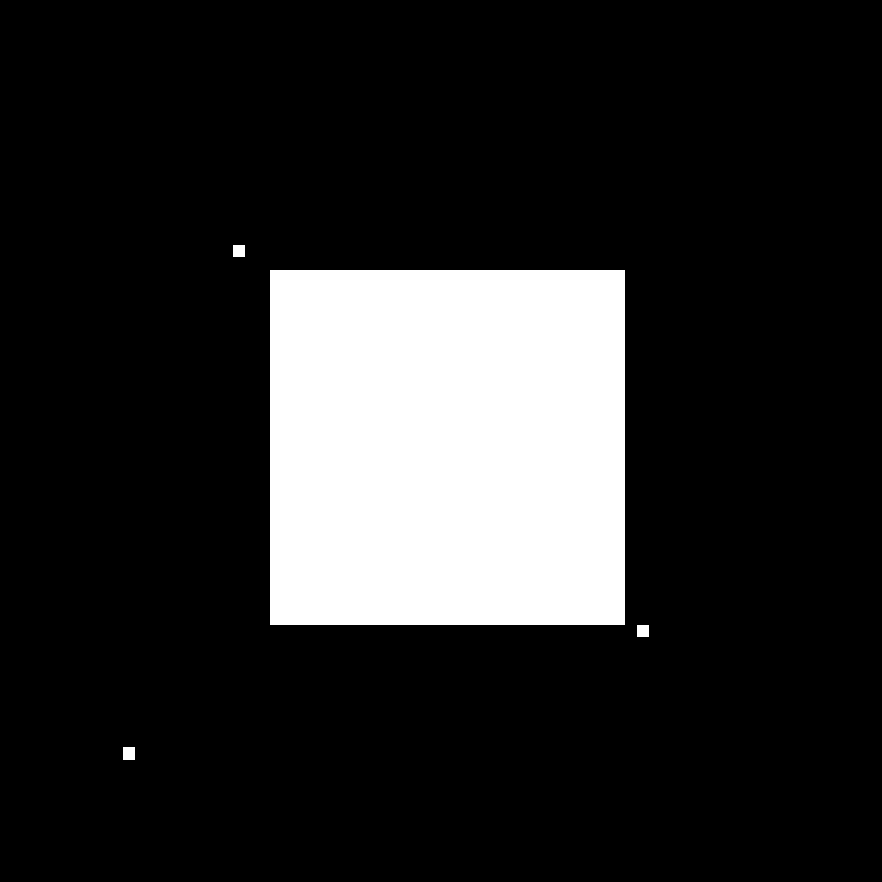
\includegraphics[width=\textwidth]{Images/Algorithm_obs/graph/Graph_explainiation_images/scene_before_graph.png}
        \caption{Scenario with salient points.}
    \end{subfigure} 
    \hfill
    \begin{subfigure}{0.3\textwidth}
        \centering
        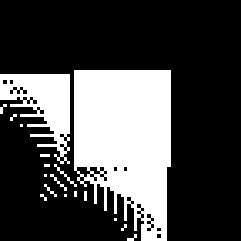
\includegraphics[width=\textwidth]{Images/Algorithm_obs/graph/Graph_explainiation_images/scene_after_graph_generation.png}
        \caption{Graph Generation.}
    \end{subfigure}
    \hfill
    \begin{subfigure}{0.3\textwidth}
        \centering
        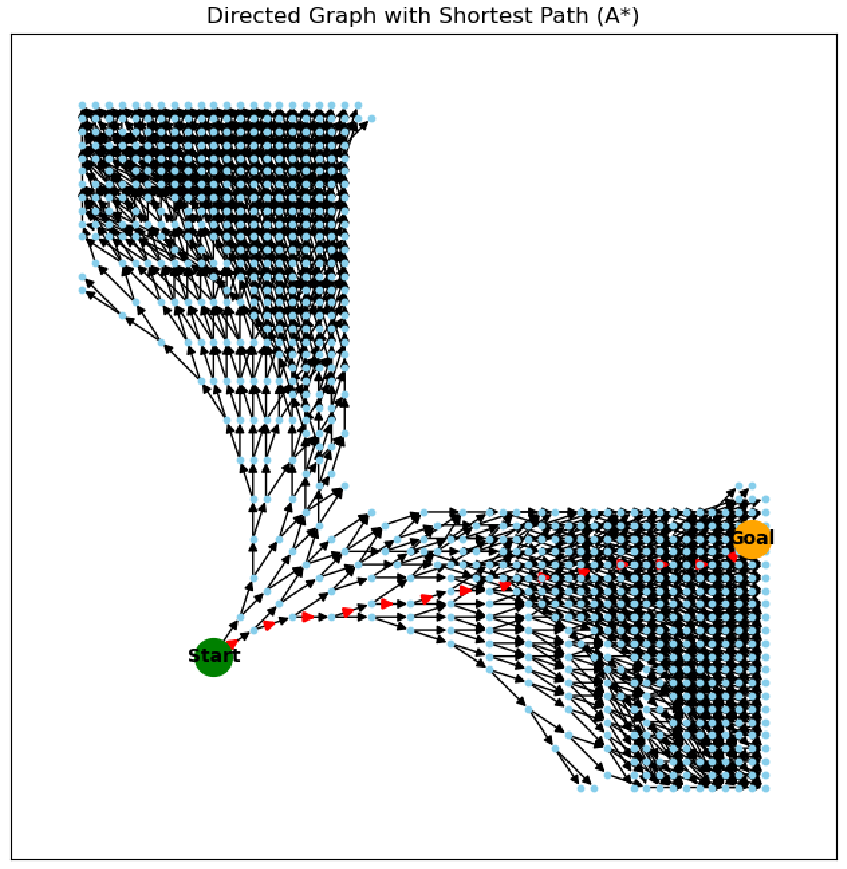
\includegraphics[width=\textwidth]{Images/Algorithm_obs/graph/Graph_explainiation_images/path.png}
        \caption{A* Search.}
    \end{subfigure}
    \caption{Graph Generation and Search.\label{fig:graph_generation}} 
\end{figure}

If the generated graph does not include the goal point, indicating that the goal point is unreachable within the constraints, the algorithm retraces one step back in the path. It then repeats the process from the point where the obstacle was detected, ensuring that the robot can circumvent the obstacle and complete its coverage path planning seamlessly.

\vspace{3mm}  

The pseudocode for path validity check and finding obstacle free path is shown in (Algorithm \autoref{alg:compute_obstacle_free_path}) .

Description of the notations:
\begin{multicols}{2}
\begin{itemize}[noitemsep,topsep=0pt]
    \item $obs\_idx$: obstacle index.
    \item $S_l$: Graph step length.
    \item $gen_{max}$: Maximum generation for graph.
    \item $P_{sh}$: Shortest path.
\end{itemize}
\end{multicols}

\begin{algorithm}[H]
    \caption{ComputeObstacleFreePath}
    \label{alg:compute_obstacle_free_path}
    \begin{algorithmic}[1]
    \Statex \textbf{Input:} Extended obstacles ($OB_e$), grids ($g_s$), buffer points ($p_{bu}$), complete path ($P_c$), current path ($P_{cu}$), current orientation ($O_{cu}$)
    \Statex \textbf{Output:} Obstacle-free path ($P_{OB free}$)
    \newline
    \State $r_{pos} \leftarrow P_{cu}[-1]$
    \State $is\_path\_in\_obstacle, obs\_idx \leftarrow$ CheckPath($P_{cu}$, $OB_e$)
    \If{$is\_path\_in\_obstacle$}
        \State $OB\leftarrow OB_e[obs\_idx]$
        \State $g \leftarrow g_s[obs\_idx]$
        \State $SP \leftarrow$ ExtractSalientPoints($OB$, $g$, $p_{bu}$, $r_{pos}$)
        \State $G.\text{initialize}()$
        \State $S_l \leftarrow$ AutoSelectStepLength($r_{pos}$, $SP$)
        \State $G$, $goal\_SP$, $is\_goal\_found \leftarrow$ GenerateGraph($G$,$r_{pos}$,$SP$,$S_l$,$gen_{max}$)
        \If{$is\_goal\_found$}
            \State $P_{sh} \leftarrow$ AStarSearch($G$,$r_{pos}$, $goal\_SP$)
            \State $P_{OB free} \leftarrow P_{sh}$
            \State \Return $P_{OB free}$
        \Else
            \State $r_{pos} \leftarrow P_c[-1]$ \Comment{Move one step back in the path}
            \State \textbf{goto} GenerateGraph (step 9)
        \EndIf
    \Else
        \State \Return $[[P_{cu}[-1], O_{cu}]]$
    \EndIf
    \end{algorithmic}
    \end{algorithm}


This iterative process repeats each time an obstacle is encountered, enabling the robot to efficiently navigate around obstacles and reach its designated goal points. This comprehensive approach ensures robust obstacle avoidance within the coverage path planning algorithm, facilitating efficient and timely completion of tasks.

\vspace{3mm}  

One last change in the complete coverage with obstacles as compared to the regular coverage is replacing the DOTSP algorithm with another algorithm that can compute path for the remaining points left near the obstacles. Since, after the behavior 2, in this case there will be only some points left that will be close to the obstacles. This happens if the points are quite close to the obstacles. Path through this points cannot be computed through DOTSP algorithm as it collides with the obstacle and path validity is not available with DOTSP. Hence, a new algorithm is introduced to compute path through these points that are close to the obstacles.  

\vspace{3mm}  

This algorithm first associate each point to its nearest obstacle. Then, we will end up with each obstacles assciated with some points. Then, the algorithm first generates the visibility graph for each obstacle with points. Then, it will find the shortest path covering all the points of first obstacle. Then, it will move to the next obstacle and cover all the points of that obstacle efficiently and so on. Eventually, it will cover all the remaining points close to all the obstacles. However, When dubins constraints are applied to this straight obstacle free path, some of the crves intersects with the corners of the obstacles due to looping of the path caused by the closeness of the points. This can be visualized in the \autoref{fig:path_around_obstacles}.


\vspace{3mm}  

The pseudocode for this path finding for remaining points is shown in (Algorithm \autoref{alg:path_around_obstacles_algorithm}). 



Notations:
\begin{itemize}[noitemsep,topsep=0pt]
    \item $P_{list}$: Points list
    \item $P_{cu}$: Current points
    \item $P_{cov}$: path through all points close to one obstacle.  
\end{itemize}

\begin{algorithm}[H]     
    \caption{PathAroundObstaclesAlgorithm}  
    \label{alg:path_around_obstacles_algorithm}
    \begin{algorithmic}[1]
    \Statex \textbf{Input:} Extended obstacles ($OB_e$), 2D points ($P_{2d}$), robot pose ($r_{pos}$), turning radius ($R_{tu}) $
    \Statex \textbf{Output:} Path ($P$)
    \newline
    
    \State $p_{list}, robot\_obs\_idx \leftarrow$ PointsCloseToObstacle($OB_e$, $P_{2d}$)
    \State $p_{cu} \leftarrow p_{list}[robot\_obs\_idx]$    \Comment{Robot close to an obstacle will be the first.}
    \State $OB_{cu} \leftarrow OB_e[robot\_obs\_idx]$
    \State $P \leftarrow []$
    \For{$i$ \textbf{in} range(len($OB_e$))}
        \State $G.\text{initialize}()$
        \State $G \leftarrow$ GenerateVisibilityGraph($OB_{cu}$, $p_{cu}$, $r_{pos}$)
        \State $P_{cov} \leftarrow$ CoverageGraphSearch($G$, $r_{pos}$)
        \State $P \mathrel{+}= P_{cov}$
        \State $r_{pos} \leftarrow P_{cov}[-1]$
        \State $OB_{cu}, obs\_idx \leftarrow$ FindNearestObstacle($r_{pos}$, $p_{list}$)
        \State $p_{cu} \leftarrow p_{list}[obs\_idx]$
    \EndFor
    \State \Return $P$
    \end{algorithmic}
    \end{algorithm}


The obstacle avoidance approach in coverage path planning addresses several critical challenges with innovative solutions. These include dynamic grid selection to balance computational complexity and accuracy, employing a hybrid space approach to represent obstacles, and optimizing computational time through dynamic step length determination. The algorithm dynamically adjusts step length based on the distance to the salient point, ensuring near-optimal path planning efficiency. Additionally, utilizing both continuous and discrete spaces allows for efficient representation of obstacles. Moreover, employing an A* search algorithm facilitates the determination of the optimal shortest path, enabling swift and effective obstacle avoidance. These integrated strategies ensure robust obstacle avoidance within the coverage path planning algorithm, enhancing overall efficiency and effectiveness.


\vspace{3mm}   


The flowchart of the complete behavioal algorithm with obstacles can be visualized in the (\autoref{fig:ccp_flowchart_obs})


% Include an image
\begin{figure}[H]
    \centering
    \includegraphics[height=22cm, width=\textwidth]{Images/flowchart/obs_flowchart.pdf}
    \caption{CCP Behavioral Algorithm with Obstacles flowchart.}
    \label{fig:ccp_flowchart_obs} 
\end{figure} 